\section{Exploring Interleaving Space}
\label{s:design}

In order to test whether threads cause a concurrency bug or not, the
straightforward method is to run the threads iteratively while
\textit{diversifying thread interleaving across iterations} until the
threads \textit{do not expose new interesting thread interleaving}.


In this section, we describe our approach to effectively explore the
search space of thread interleaving.
%
We first describe the key idea of our
approach~(\autoref{ss:overview}). Then, we illustrate our coverage
metric in the concurrency dimension~(\autoref{ss:coverage}), and the
instruction scheduling algorithm to quickly saturate the
coverage~(\autoref{ss:scheduler}).



While this section focuses only on exploring the search space of
thread interleaivng of given threads, \autoref{s:impl} describes the
whole design of \sys for expanding both code coverage and interleaving
coverage.


\subsection{Key Idea}
\label{ss:overview}

\begin{figure}[t]
  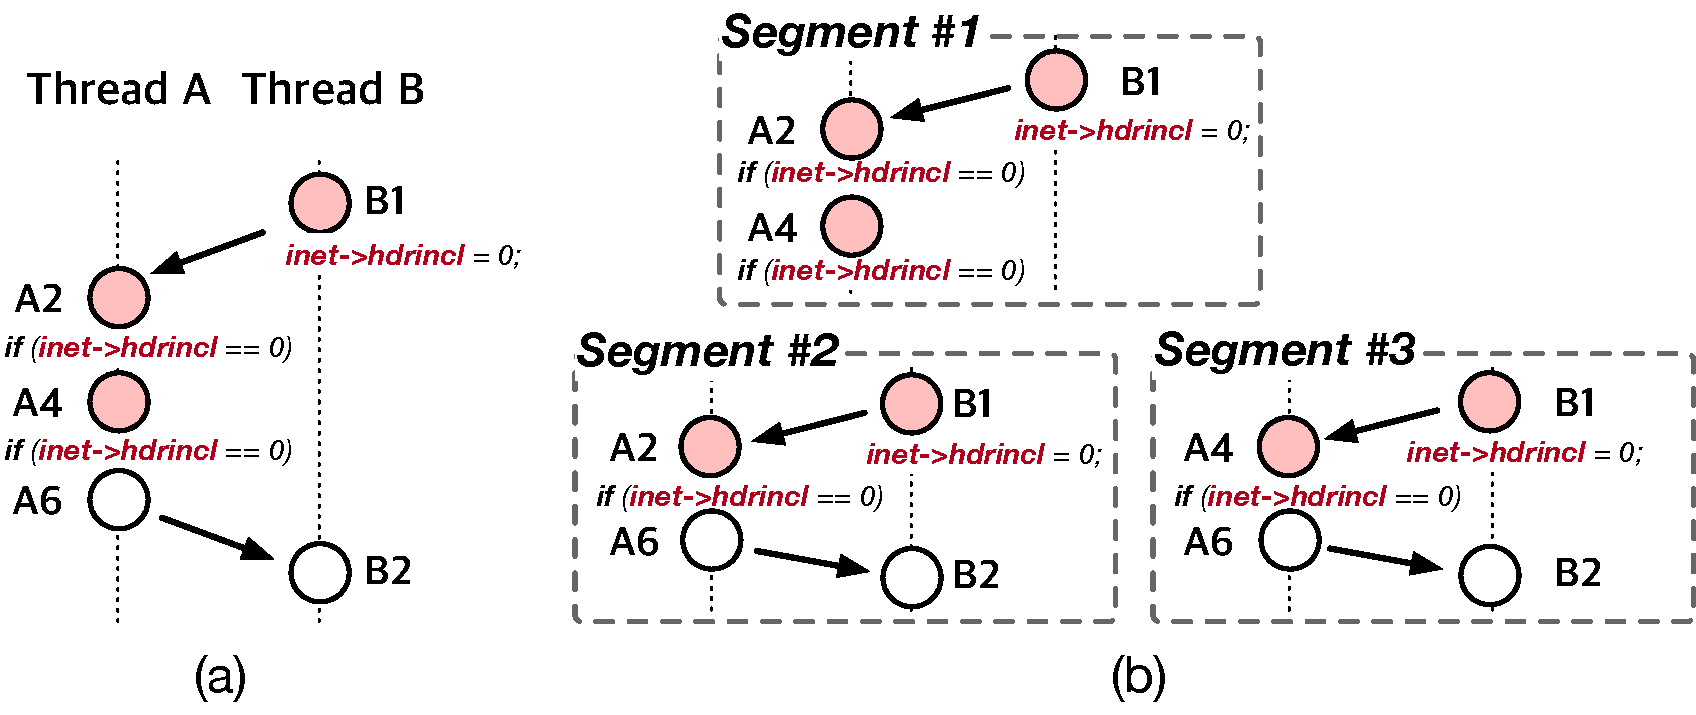
\includegraphics[width=0.9\linewidth]{fig/intuition.pdf}
  \caption{Approach overview to explore the interleaving
    space.}
  \label{fig:keyidea}
\end{figure}
%
The key idea of our approach is to consider an instance of thread
interleaving as \textit{a composition of interleaving segments}, where
each interleaving segment represents the execution order of a small
number of memory accesses.
%
In particular, after executing threads concurrently, we firstly model
an execution of these threads as a totally-ordered instruction
sequence.
%
And then, we group a small number of instructions (\eg, four
instructions) as a segment to track which segments are contained in
the execution and search for other segments in future iterations.


\autoref{fig:keyidea} visualizes our key idea.
%
In this example, let us assume we are testing whether thread
interleaving of the two system calls, \texttt{Syscall A} and
\texttt{Syscall B}, causes a concurrency bug.
%
While executing the two system calls, we track memory access
operations conducted by the two system calls with timestamps, and
construct a totally-ordered instruction sequence as described in
\autoref{fig:keyidea}-(a).

we can decompose the interleaving instance into three interleaving
segments as described in \autoref{fig:keyidea}-(b).


It is worth noting that segments can be overlapped; in this example,
\texttt{Segment \#1} and \texttt{Segment \#2} are overlapped over XXX.





\PP{Benefits}
%
This approach provides two remarkable benefits.
%
\textbf{i)} Tracking interleaving segments is a befitting choice to
determine if any \textit{interesting} thread interleaving remains.
%
According to the extensive survey conducted by Shan Lu
\etal~\cite{learningfrommistakes}, most (\ie, more than 90\%)
concurrency bugs manifest depending on the execution order of a small
number (mostly, four) of memory accesse.
%
In this perspective, whether or not an interleaving instance causes a
concurrency bug depends on whether a problematic segment is contained
in the instance of thread interleaving.
%

\textbf{ii)} interleaving segments contained in an iteration gives
promising hints for diversifying thread interleaving in future
iterations.
%
In other words, with a given interleaving segment, we can rearrange
instructions in the interleaving segment to derive \textit{unobserved}
interleaving segment.

\begin{figure}[t]
  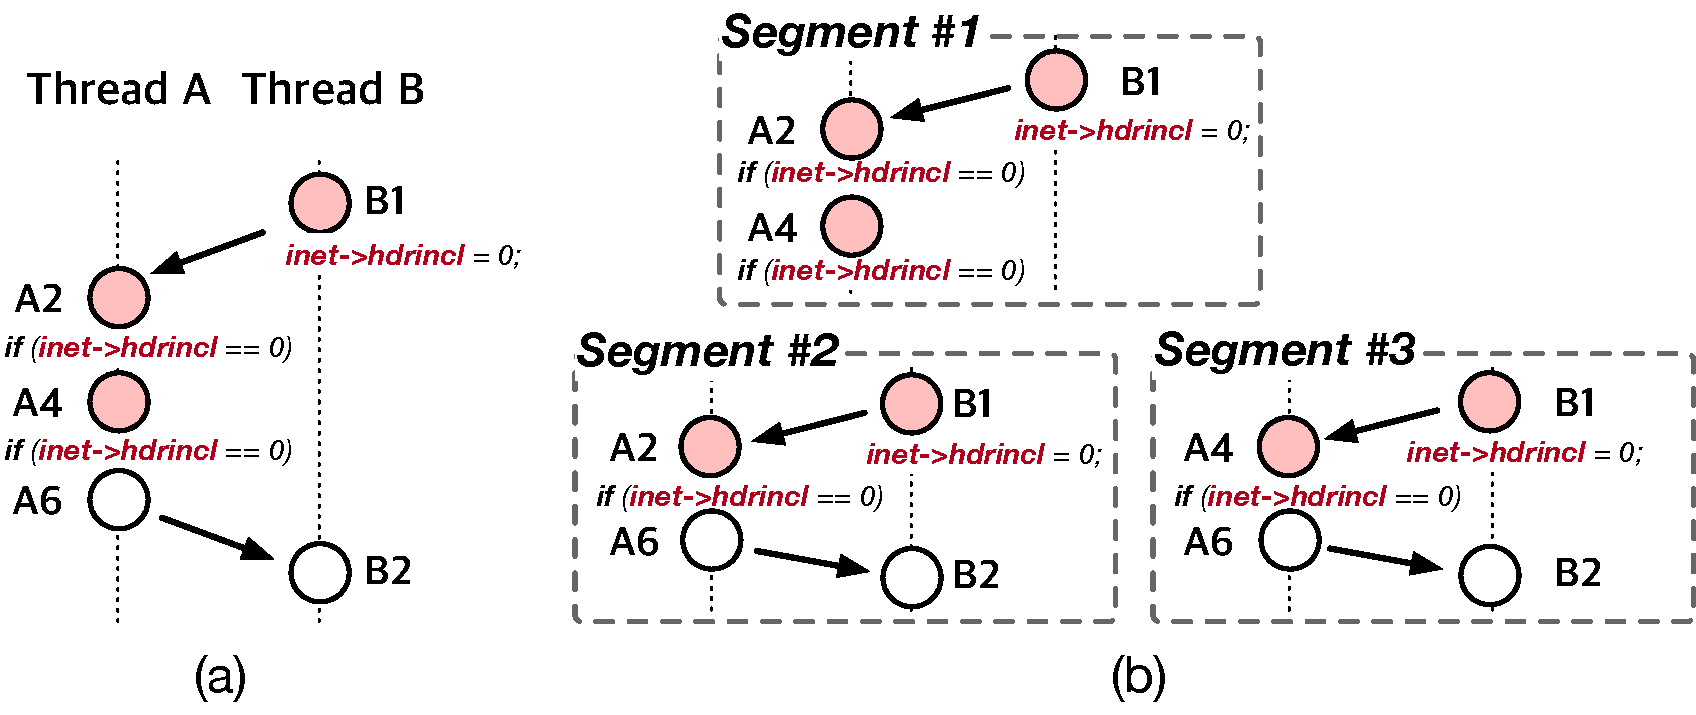
\includegraphics[width=0.9\linewidth]{fig/intuition.pdf}
  \caption{Approach overview to explore the interleaving
    space.}
  \label{fig:hint}
\end{figure}
%
\autoref{fig:hint} 


\subsection{Interleaving Segment Coverage}
\label{ss:coverage}

Based on the key idea, we propose a novel coverage in the concurrency
dimension called interleaving segment coverage.
%



\newcommand{\mutable}{mutable edge\xspace}
\newcommand{\mutables}{mutable edges\xspace}
\newcommand{\immutable}{immutable edge\xspace}
\newcommand{\immutables}{immutable edges\xspace}
%
Biconflict converage is designed to track conjunctions of scheduling
constraints, and if per-input biconflict coverage is saturated, we
confidently conclude that the concurrent job unlikely causes a race
condition.

We track biconflict coverage \textit{offline}\yj{I do not get it}. During the runtime of a
kernel, the fuzzer only collects memory access operations conducted by
the concurrent job (\eg, syscalls), and after executing the concurrent
job, the fuzzer measures biconflict coverage of the concurrent job.

\PP{Definition of biconflict coverage}
%
Let us represent a memory access operation $M$ as four tuples,
$(tid, addr, op, timestamp)$ where $tid$ is the identity of a thread,
$addr$ is the address of a memory location, $op$ is the type of the
memory access operation (\ie, $store$ or $load$), and $timestamp$
indicates the point of time when the memory access operation is taken.
%
$M(x)$ detnoes a field $x$ of $M$. For example, $M(tid)$ is a $tid$
field of a memory access operation $M$.
%
Also let us suppose all memory access operations are totally
ordered. \ie, there are no two memory access operations that have the
same $timestamp$.

For all pair of memory access operations $M_i$ and $M_j$, we define a
scheduling constraint $SC$ as a tuple $(M_i, M_j)$ if
$M_i(tid) \neq M_j(tid)$, $M_i(addr) = M_j(addr)$,
$M_i(op) = store \vee M_j(op) = store$, and
$M_i(timestamp) < M_j(timestamp)$.
%
Informally, $M_i$ and $M_j$ are conflicting memory acceess operations
that are executed in other threads, and $M_i$ was taken place before
$M_j$.
%
For two scheduling constraint $SC_1(M_{1i}, M_{1j})$ and
$SC_2(M_{2i}, M_{2j})$, $SC_1 = SC_2$ if
$(M_{1i} = M_{2i}) \wedge (M_{1j} = M_{2j})$.
%
Then, we define a scheduling constraint pair $SCPair = (SC_i, SC_j)$
for two scheduling constraints if $i < j$, $SC_i \neq SC_j$.
%
Lastly, biconflict coverage of the concurrent job $BC\mbox{-}Cov$ is
defined as a set of all scheduling constraint pairs,
$\{SCPair_1, SCPair_2, ..., SCPair_n\}$, constructed from its memory
access operation sequence.



\PP{Predicting potential biconflict coverage}
%
An interleaving finding new biconflict coverage likely exposes a
behavior that was unrevealed before.
%
To discover more interesting behaviors, if new biconflict coverage is
found, the fuzzer mutates the interleaving. \ie, the fuzzer
reschedules instructions to conform with other interleavings.

Before mutating an interleaving, the fuzzer predicts \textit{potential
  biconflict coverage}, $BC\mbox{-}Cov^*$, a set of scheduling
constraint pairs that \textit{has not been observed but is expected to
  occur with other interleavings}.
%
Potential binconflict coverage will be used to direct the interleaving
mutation. \ie, the fuzzer will try to generate interleavings to expose
undisclosed scheduling constraint pairs contained in
$BC\mbox{-}Cov^*$, instead of blindly mutating an interleaving.


$BC\mbox{-}Cov^*$ is derived from biconflict coverage $BC\mbox{-}cov$,
$\{SCPair_1, SCPair_2, ..., SCPair_n\}$.
%
For each $SCPair_i$ composed of $(SC_x, SC_y)$ in $BC\mbox{-}cov$, the
fuzzer derives \dr{TODO}...



\subsection{Coverage-directed Interleaving Mutation}
\label{ss:scheduler}


%%% Local Variables:
%%% mode: latex
%%% TeX-master: "p"
%%% End:
